\hypertarget{bch-and-rs}{%
\section{BCH and RS}\label{bch-and-rs}}

\hypertarget{hamming-code}{%
\subsection{Hamming Code}\label{hamming-code}}

\begin{itemize}
\tightlist
\item
  Every code word consists of $n = 2^m - 1$ binary digits

  \begin{itemize}
  \tightlist
  \item
    $u = (u_0 , u_1 , \ldots{}, u_{n-1} )$
  \end{itemize}
\item
  Die möglichen Code-Wörter lassen sich auch als Polynome darstellen.
\item
  Der Grad des Polynoms ist $m$
\item
  Die Anzahl binärer Vektoren bzw. die Anzahl Code-Symbole $n$ ist gleich
  $n = 2^m - 1$
\item
  Für die Rechnung im binären Raum wird die binäre Schreibweise der
  Polynome verwendet
\end{itemize}

\begin{figure}[H]
\centering
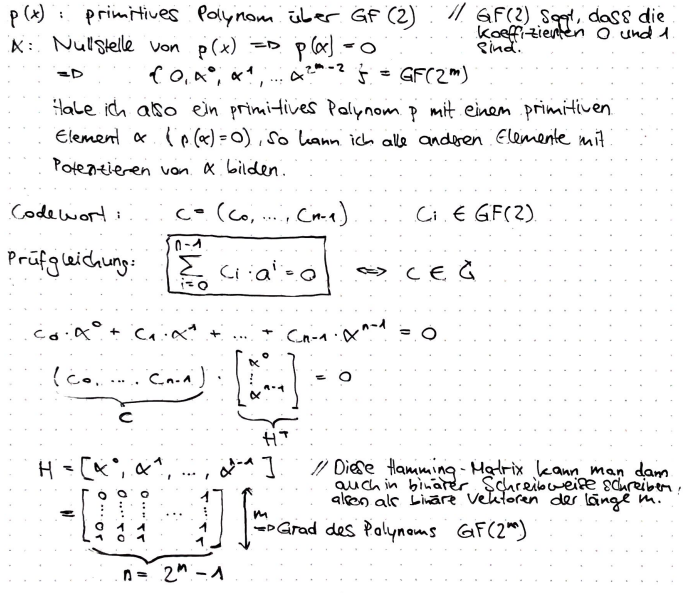
\includegraphics[width=0.8\textwidth]{figures/hamming-code.png}
\caption{Hamming Code Notes}
\end{figure}

\hypertarget{cyclic-hamming-code}{%
\subsection{Cyclic Hamming Code}\label{cyclic-hamming-code}}

\begin{figure}[H]
\centering
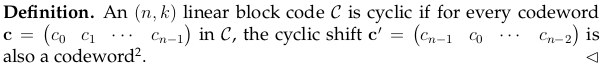
\includegraphics[width=0.8\textwidth]{figures/definitionCyclicHamming.png}
\caption{Definition Cyclic Hamming Code}
\end{figure}

\begin{itemize}
\tightlist
\item
  Der Code ist als Polynom geschrieben
\item
  Um das Code-Wort an der Stelle X zu bekommen, setzt man für X ein Wert
  ein (in diesem Fall a)
\item
  The primitive polynomial $m(X)$ is the polynomial of \textbf{smallest
  degree} $m = n - k$ having the primitive element $a$ as root

  \begin{itemize}
  \tightlist
  \item
    Every code polynomial $u(X)$ must be a multiple of $m(X)$
  \item
    The primitive polynomial $m(X)$ of degree m is the generator
    polynomial $g(X)$ of the cyclic ($2^m - 1, 2^m - m - 1$)-Hamming
    code
  \end{itemize}
\end{itemize}

\begin{figure}[H]
\centering
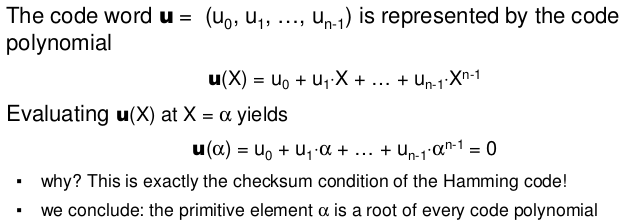
\includegraphics[width=0.7\textwidth]{figures/cyclicHammingCode.png}
\caption{Cyclic Hamming Code Slide}
\end{figure}

\hypertarget{bose-chaudhuri-hocquenghem-bch}{%
\subsection{Bose-Chaudhuri-Hocquenghem
(BCH)}\label{bose-chaudhuri-hocquenghem-bch}}

\begin{itemize}
\tightlist
\item
  Wie beim Hamming Code wählen wir ein Körper $GF(2^m)$
\item
  Und wir suchen ein primitives Element $a$
\item
  Die Anzahl Code-Symbole $n$ ist ebenfalls wieder $n = 2^m -1$
\item
  Wir führen jedoch eine weitere Verschärfung $q$ in der Checksumme ein.
\item
  Die Prüfsumme muss also auch für jedes $q$ von $1$ bis $r$ stimmen
\item
  $r$ bestimmt die Anzahl Fehler, die korrigiert werden können
\item
  Für den normalen Hamming-Code ist $ = 1$ also $r = 1$, er kann nur einen
  Fehler korrigieren
\end{itemize}

\begin{figure}[H]
\centering
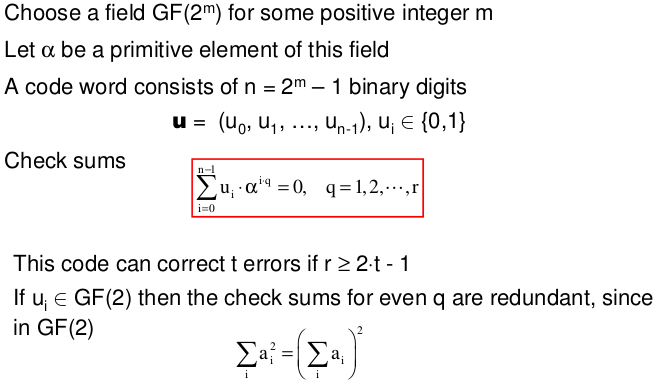
\includegraphics[width=0.55\textwidth]{figures/bch.png}
\caption{BCH Slides}
\end{figure}

\begin{itemize}
\tightlist
\item
  Im $GF(2)$ gilt die komische Regel, dass die Summe aller Quadrate
  dasselbe ist die das Quadrat der Summe
\item
  Aus diesem Grund muss ich nur die ungeraden $q$ überprüfen, da für jedes
  gerade $q$ dasselbe gilt
\item
  Aus diesem Grund haben wir auch die zweite Bedingung in der folgenden
  Parity Check Matrix gestrichen
\end{itemize}

\begin{figure}[H]
\centering
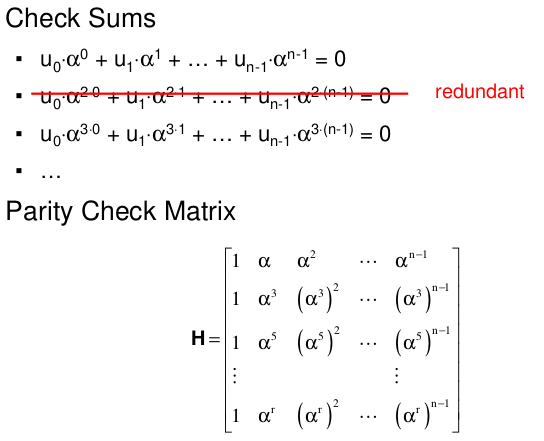
\includegraphics[width=0.5\textwidth]{figures/bch2.png}
\caption{BCH Slides 2}
\end{figure}

\hypertarget{example}{%
\subsubsection{Example}\label{example}}

\begin{figure}[H]
\centering
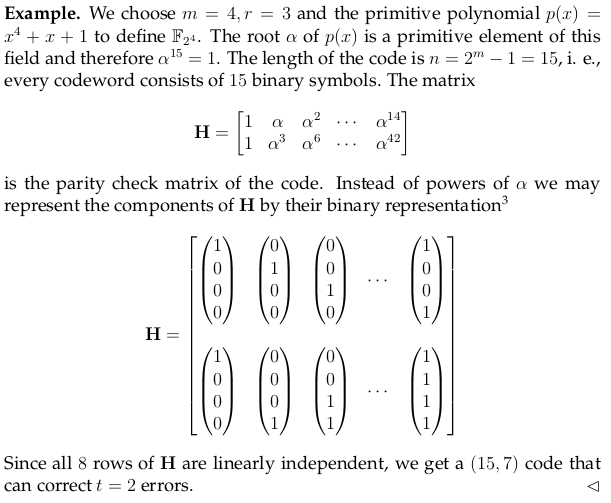
\includegraphics[width=0.75\textwidth]{figures/bchExample.png}
\caption{BCH Example}
\end{figure}

Note that in this field we have $a^6 = a^3 + a^2 , a^{14} = a^3 + 1 and a^{42} =
a^{12} = a^3 + a^2 + a + 1$

\begin{tcolorbox}[colback=red!5!white,colframe=red!75!black]
Achtung: Es kommt nicht darauf an, ob in der Prüfmatrix die binären Koeffizienten von unten oder von oben beginnen, also ob $a^0 = 0001$ oder $a^0 = 1000$ ist
\end{tcolorbox}

\begin{figure}[H]
\centering
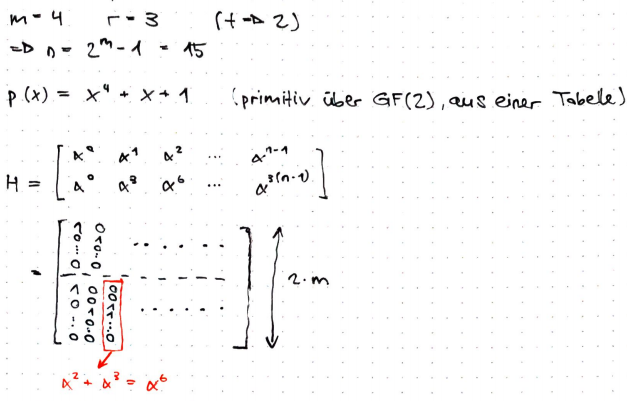
\includegraphics[width=0.7\textwidth]{figures/bch-Example.png}
\caption{BCH Example}
\end{figure}

\begin{figure}[H]
\centering
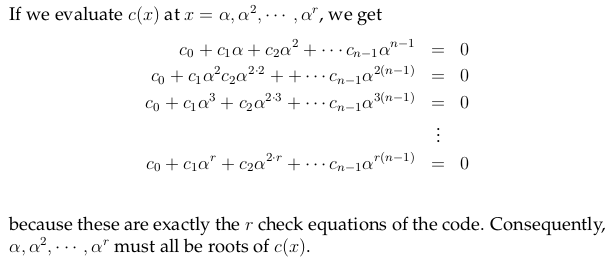
\includegraphics[width=0.8\textwidth]{figures/bchRequirement2.png}
\caption{BCH Requirements 2}
\end{figure}

\hypertarget{generator-polynomial}{%
\subsection{Generator Polynomial}\label{generator-polynomial}}

\textbf{Definition}: The unique monic nonzero code polynomial of minimum
degree in a cyclic code C is called the generator polynomial of C and is
denoted by $g(x)$.

\textbf{Definition}: Das minimalste Polynom von $\beta$ in $GF(p^n)$ ist
definiert durch:\\
Das kleinst mögliche monische Poloynom mit Koeffizienten in $GF(p)$ das $\beta$ als Nullstelle hat.

\begin{itemize}
\tightlist
\item
  Wenn ich ein Generator Polynom suche, das alle möglichen Alphas als
  Nullstelle hat, muss ich zuerst von allen Alphas das minimalste
  Polynom berechnen
\item
  Wenn ich alle minimalsten Polynome habe, kann ich das Generator
  Polynom berechnen, in dem ich die verschiedenen minimal Polynome
  miteinander multipliziere
\end{itemize}

\begin{figure}[H]
\centering
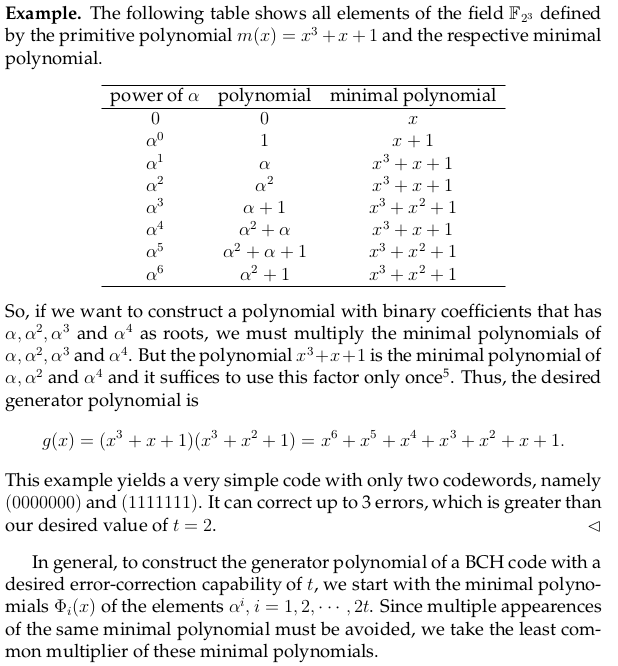
\includegraphics[width=0.7\textwidth]{figures/generatorPolynomial2.png}
\caption{Generator Polynom - Slides 1}
\end{figure}

\begin{itemize}
\tightlist
\item
  Phi ist in diesem Fall das minimalste Polynom von Alpha. Das Generator Polynom
  berechne ich mit der Multiplikation aller verschiedenen Phis (deswegen
  das lcm vor der Klammer)
\end{itemize}

\begin{figure}[H]
\centering
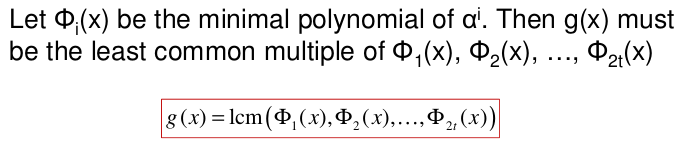
\includegraphics[width=0.6\textwidth]{figures/generatorPolynomial3.png}
\caption{Generator Polynom - Slides 2}
\end{figure}

\clearpage

\textbf{Grund für dieses Vorgehen:}

\begin{figure}[H]
\centering
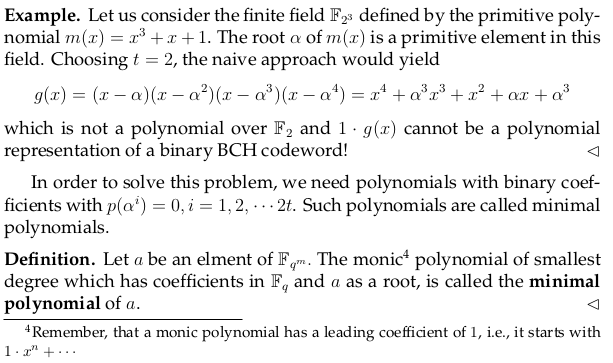
\includegraphics[width=0.6\textwidth]{figures/generatorPolynomial.png}
\caption{Generator Polynom - Slides 3}
\end{figure}

\hypertarget{reed-solomon-codes}{%
\subsection{Reed Solomon Codes}\label{reed-solomon-codes}}

\begin{itemize}
\tightlist
\item
  Non-binary BCH codes
\item
  Ein Code-Wort besteht aus $n$ Symbolen, aber alle Symbole stammen von
  einem Körper $GF(q)$
\item
  Usually $q = 2^m$

  \begin{itemize}
  \tightlist
  \item
    each code symbol can be represented by a binary vector of length $m$
  \end{itemize}
\item
  A code word consists of $n = q - 1$ code symbols
\end{itemize}

\hypertarget{discrete-fourier-transform---dft}{%
\subsubsection{Discrete Fourier Transform -
DFT}\label{discrete-fourier-transform---dft}}

\begin{itemize}
\tightlist
\item
  Sie haben irgendeinen Vektor klein $v$, mit $n$ Elementen
\item
  Daraus möchten wir einen Vektor gross $V$ bauen, mit $n$ Elementen
\item
  Mit der entsprechenden Formeln
\end{itemize}

\begin{figure}[H]
\centering
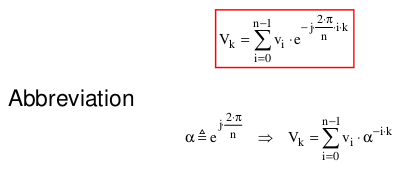
\includegraphics[width=0.5\textwidth]{figures/dft.png}
\caption{DFT}
\end{figure}

\begin{itemize}
\tightlist
\item
  Diese Summe lässt sich dann auch als Matrix schreiben
\item
  Die Schreibweise als Matrix ist in jedem Fall gleich und man kann
  diese einfach so aufschreiben
\item
  Die Inverse Matrix lässt sich auch einfach schreiben und damit lässt
  sich z.B. auch wieder das kleine $v$ ausrechnen
\item
  Problem hier: Das n existiert in gewissen Körpern nicht.
\item
  Lösung: In unserem Fall, in dem wir immer im $GF(2)$ rechnen, ist das $n$
  immer 1 oder 0 $\Rightarrow$ 0 ist nicht erlaubt. Das heisst, wir lassen $1/n$ einfach weg.
\end{itemize}

\begin{figure}[H]
\centering
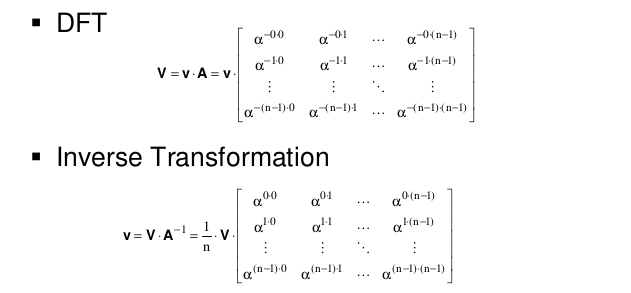
\includegraphics[width=0.6\textwidth]{figures/dftMatrixRepresentation.png}
\caption{DFT Matrix Representation}
\end{figure}

\begin{itemize}
\tightlist
\item
  Die dritte Möglichkeit, die DFT zu schreiben, ist als Polynom.
\item
  $V$ an der Stelle $k$ ist das kleine $v$ mal das Polynom an der Stelle $\alpha ^{-k}$.
\item
  Auf der anderen Seite kann ich auch das Inverse wieder berechnen, in
  dem ich das grosse $V$ mal das $\alpha$ an der Stelle $i$ rechne.
\end{itemize}

\begin{figure}[H]
\centering
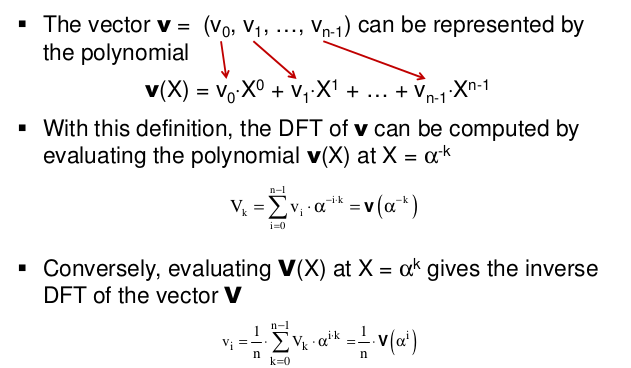
\includegraphics[width=0.5\textwidth]{figures/dftPolynomial.png}
\caption{DFT Polynomial Representation}
\end{figure}

\begin{itemize}
\tightlist
\item
  Wir können also das primivite Element Alpha im $GF(2^m)$ nehmen
\item
  Das $a^j$ ist nie 1, ausser wenn $j$ das letzte Element im Körper ist
\end{itemize}

\begin{figure}[H]
\centering
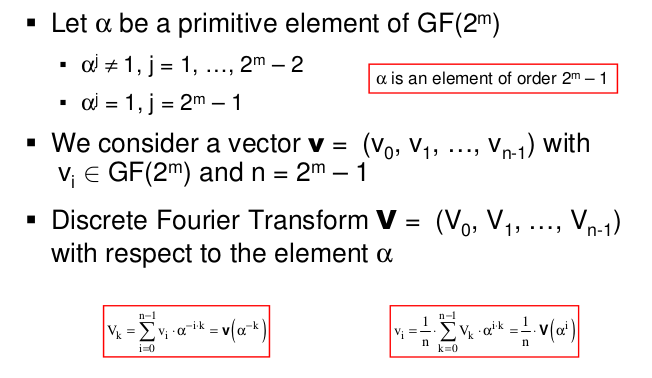
\includegraphics[width=0.5\textwidth]{figures/dftInGf2.png}
\caption{DFT in GF2}
\end{figure}

\hypertarget{reed-solomon-code}{%
\subsubsection{Reed Solomon Code}\label{reed-solomon-code}}

\begin{itemize}
\tightlist
\item
  Wir brauchen ein primitives Element im Körper $GF(q)$ also $GF(2^m)$
\item
  Das primitive Element findet man am einfachsten, wenn man ein
  primitives Polynom definiert und die Nullstelle findet
\item
  Ein Vektor $u$ ist genau dann ein Code-Wort, wenn die Fourier
  Transformation $U$ an den letzten $2*t$ Stellen 0 hat
\item
  Also wenn $t = 2$ Fehler korrigiert werden können, müssen die letzten 4
  Stellen 0 sein
\end{itemize}

\begin{figure}[H]
\centering
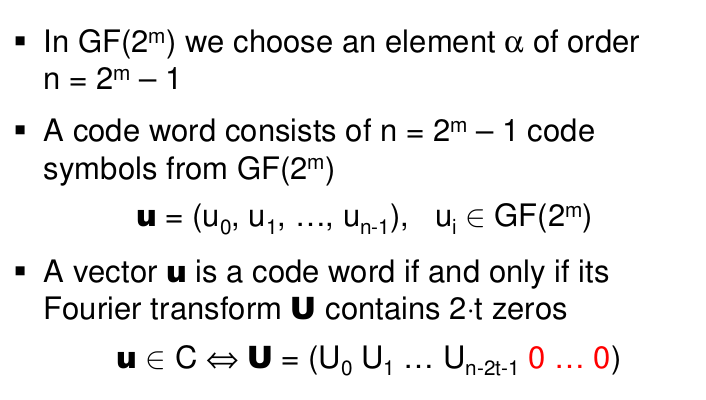
\includegraphics[width=0.5\textwidth]{figures/reedSolomonCode.png}
\caption{Reed Solomon Code - Slides 1}
\end{figure}

\begin{itemize}
\tightlist
\item
  Da wir wissen, dass $u$ an den Stellen $a^1$ bis $a^{2t}$ Nullstellen hat,
  wissen wir, wie wir das Generator-Polynom $g(x)$ generieren können
\end{itemize}

\begin{figure}[H]
\centering
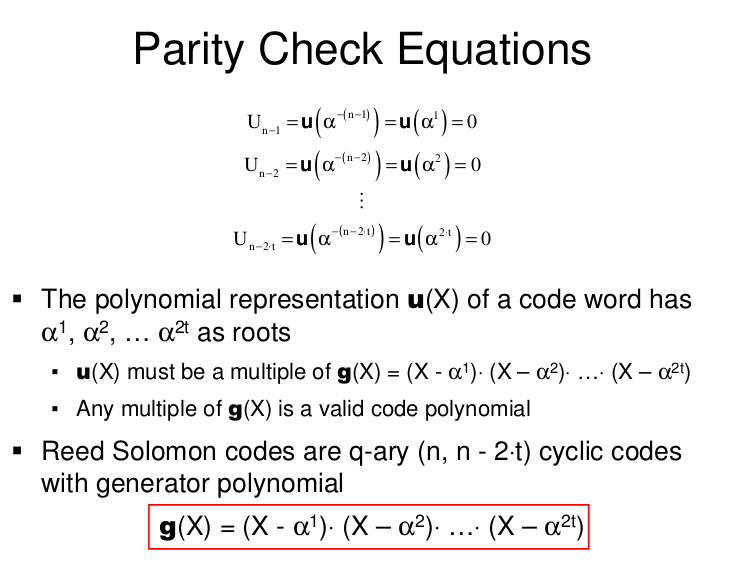
\includegraphics[width=0.5\textwidth]{figures/reedSolomonCode2.png}
\caption{Reed Solomon Code - Slides 2}
\end{figure}

\hypertarget{decoding}{%
\subsubsection{Decoding}\label{decoding}}

\begin{itemize}
\tightlist
\item
  Wir empfangen $r$, das ist das gesendete $u$ + ein Fehler $e$
\item
  Da die DFT linear ist, ist gross U + gross E immer noch gross R
\item
  Uns interessieren eigentlich nur die letzten 2t Stellen von gross R
\item
  Sind diese 0, ist das Code-Wort R gültig
\end{itemize}

\begin{figure}[H]
\centering
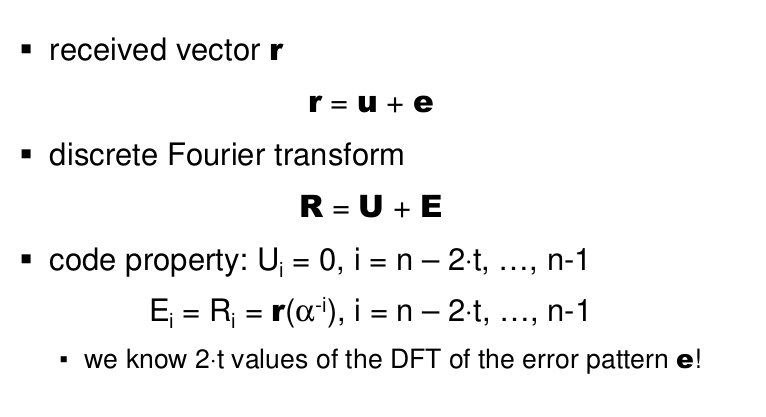
\includegraphics[width=0.5\textwidth]{figures/reedSolomonDecoding.png}
\caption{Reed Solomon Code - Slides 3}
\end{figure}

\begin{itemize}
\tightlist
\item
  Falls das Fehlermuster $e$ höchstens $t$ Fehler enthält, können wir den
  gesamten Vektor E von den bekannten 2t Werten herstellen
\end{itemize}

\begin{figure}[H]
\centering
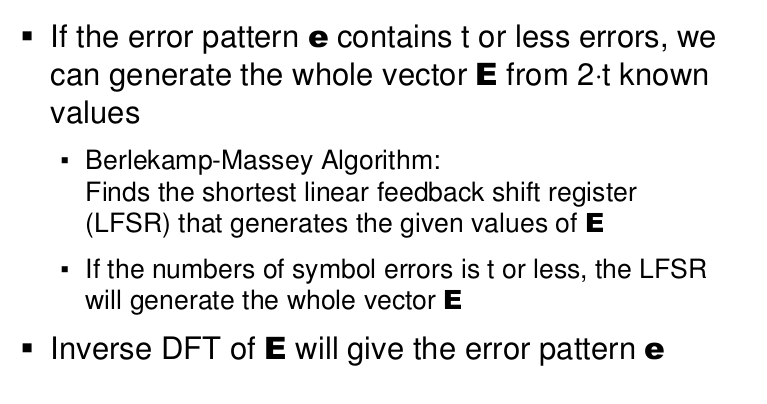
\includegraphics[width=0.5\textwidth]{figures/reedSolomonDecoding2.png}
\caption{Reed Solomon Code - Slides 4}
\end{figure}

\begin{itemize}
\tightlist
\item
  Ich berechne gross R mit dem DFT des empfangenen r
\item
  Mich interessieren dann nur noch die letzten 2t Stellen von R
\item
  Falls die Anzahl Fehlerbits maximal t sind, kann ich mit dem
  Massey-Berlekamp Algorithmus das Linear Feedback Shift Register
  durchführen und erhalte gross E
\item
  Mit dem inversen DFT von E erhalte ich das Error-Pattern e
\end{itemize}

\begin{figure}[H]
\centering
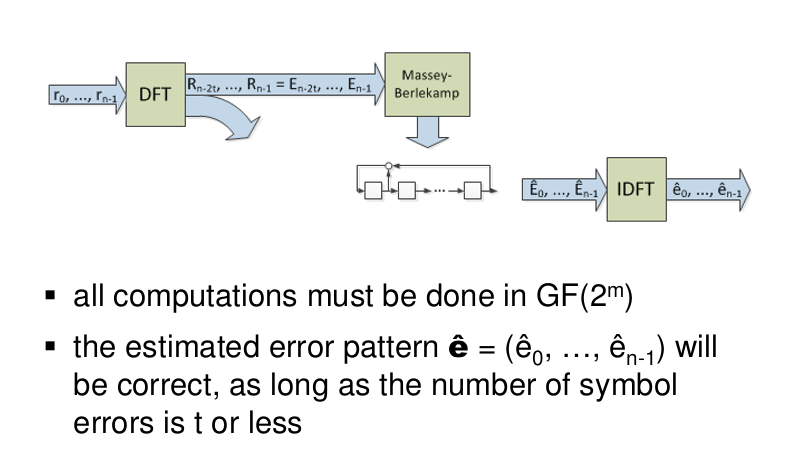
\includegraphics[width=0.55\textwidth]{figures/reedSolomonDecoding3.png}
\caption{Reed Solomon Code - Slides 4}
\end{figure}

\hypertarget{decoding-algorithm-vom-script}{%
\subsubsection{Decoding Algorithm vom
Script}\label{decoding-algorithm-vom-script}}

\begin{enumerate}
\tightlist
\item
  Compute the DFT R of the received vector $r$.
\item
  The last $2t$ values of R are identical to the last $2t$ values of $E$.
\item
  Find the shortest LFSR that generates the known values of $E$. This
  problem is solved by the Massey-Berlekamp algorithm.
\item
  Use this LFSR to generate $n$ values of $E$ and shift them cyclically to $e$
  get the vector $e'$.
\item
  Compute the inverse DFT of $E'$. This will yield the estimate of the
  error pattern $e'$.
\item
  Correct the received data by computing $c' = r - e'$.
\end{enumerate}

\clearpage
